\section{Sensor Rig Design}
The sensor rig is designed to be carried and operated by a single person but can also be attached to a vessel.
Two 1m carbon fiber tubes serve as the main structure, providing rigidity to the rig without adding much weight.
Except for the waterproof enclosure and the two carbon fiber tubes, all the mechanical parts are 3D printed, making the sensor rig easy to reproduce and modify.
The various parts are designed to clamp onto the \SI{30}{mm} carbon fiber tubes, and friction tape ensures a tight fit.
This makes it easy to extend the rig with additional sensors or design various clamping brackets to attach it to different vessels.
An IP67-rated waterproof enclosure protects the internal electronics from the elements, allowing for operation in different weather conditions.
The components inside the enclosure are mounted on two detachable 3D-printed plates locked in place by a wedge system. This makes it easy to remove and replace the internal components if needed.
The choice of components dominates the weight and cost of the sensor rig, which can be adjusted to fit the user's needs.
With the current components and battery, it weighs \SI{5.75}{kg} in total.

\begin{figure}[H]
    \centering
    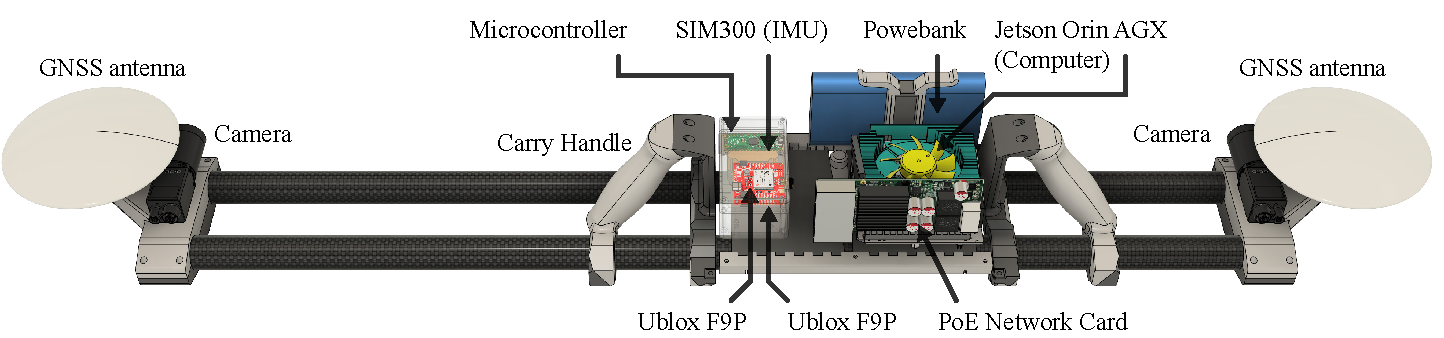
\includegraphics[width=\textwidth]{figures/rig_components.pdf}
    \caption{Cad model of the sensor rig with the enclosure removed for visibility.}
\end{figure}

\subsection{Components}
In its current configuration, one TRI050S1-QC polarization camera and one TOP106 L1/L2 GNSS antenna are mounted on each side of the sensor rig to provide wide baseline stereo video and differential GNSS data for accurate heading estimation.
The cameras have a 2/3" global shutter sensor with a $2448\times2048$ resolution, are equipped with an 8mm lens, and are configured to capture 12-bit raw color polarization video at \SI{14}{fps}.

Inside the waterproof enclosure, an Nvidia Jetson Orin AGX serves as the main processing unit.
The Jetson is a single-board computer designed for edge computing with a dedicated GPU, GPIO, and multiple hardware accelerators for video processing and AI \cite{karumbunathanNVIDIAJetsonAGX2022}.
An external network card is connected to the Jetson through its PCIe slot. 
It provides 4 separate \SI{1}{Gb/s} ethernet ports with \gls{poe} to power and communicate with the cameras and other sensors over a single cable, and supports \gls{ptp} synchronization.
Two F9P GNSS receivers and a STIM300 \gls{imu} provide the sensor data required for accurate pose estimation.
With a \SI{100}{Wh} detachable power bank, the sensor rig can record data for approximately 5 hours before needing a battery change.

\begin{figure}[H]
    
    \centering
    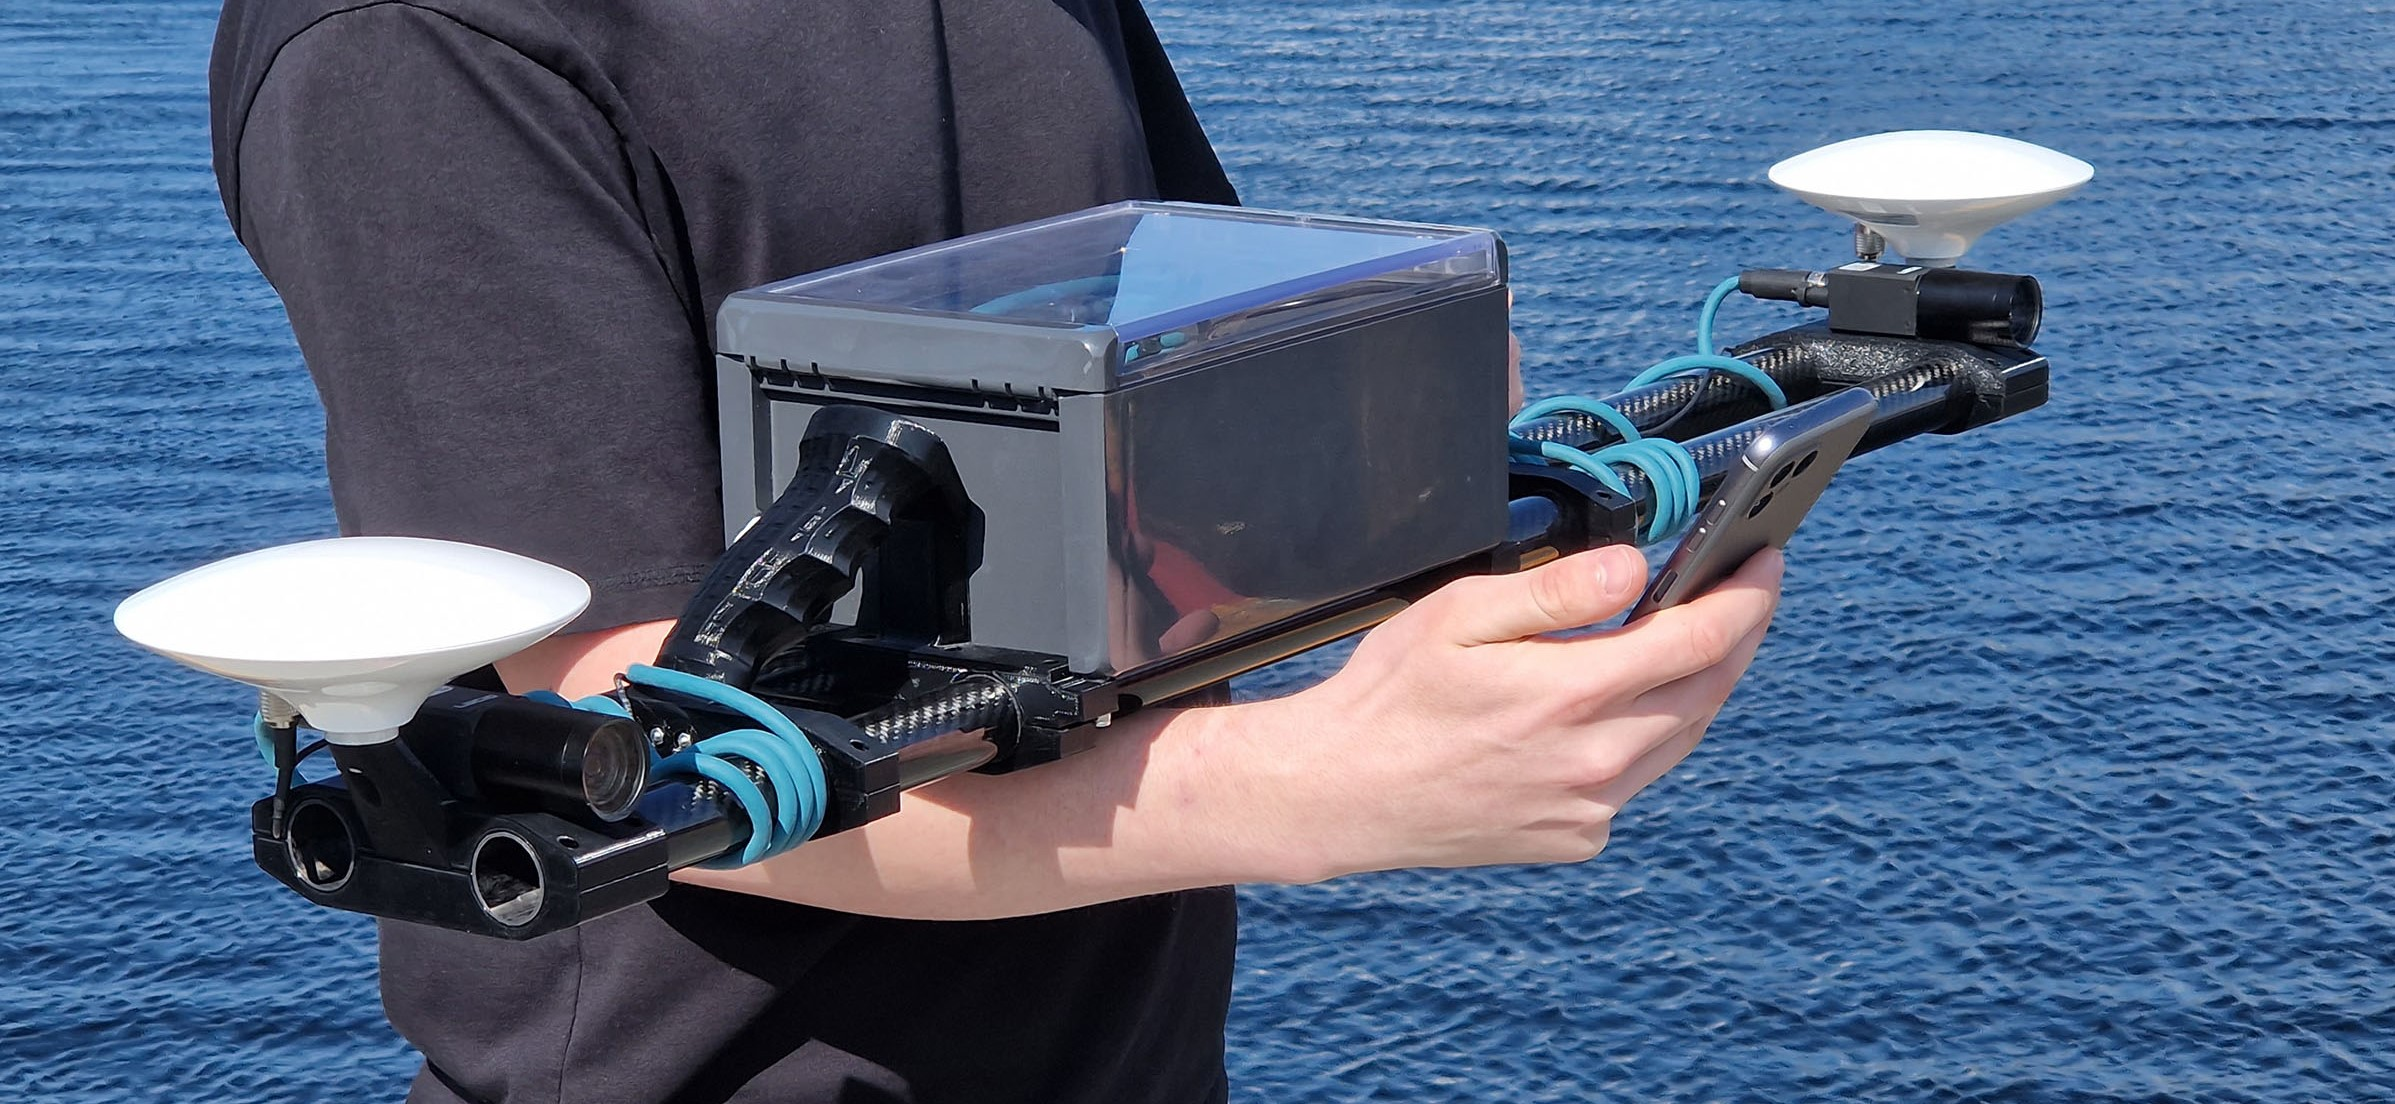
\includegraphics[trim={0 2cm 0 1cm},clip,width=\textwidth]{figures/operation.jpg}
    \caption{Human operation of the sensor rig with monitoring over a smartphone. \label{fig:operation}}
\end{figure}

\subsection{Control and Monitoring}
The sensor rig hosts a web app that allows the operator to control and monitor the data acquisition from their smartphone, as depicted in Figure \ref{fig:operation}.
The web app is built with SvelteKit and communicates with the different programs running on the Jetson through WebSockets.
From the app, the operator can start and stop the acquisition, view incoming data from the different sensors, and view a live stream from the cameras.
The app also provides information from the Jetson, such as CPU temperature, storage usage, synchronization status, and battery voltage.
Earlier versions of the app allowed the user to configure parameters such as exposure and gain, but we noticed that this took away focus, so we switched to automatic adjustment of these parameters.
The simple interface enhances its usability and makes it possible for anyone to use the sensor rig without training.

\subsection{Sensor Synchronization}
% Emphasis has been put on accurately synchronizing all sensors on the sensor rig to \gls{utc}.
The \gls{gnss} receivers are synchronized to \gls{utc} by themselves and do not require further synchronization.
The \gls{imu} samples at a fixed frequency following an internal clock \cite{safranSTIM300Datasheet}.
When it receives a trigger signal, it sends the latest available data, the trigger count, and the delay between the latest message and the trigger \cite{safranSTIM300Datasheet}.
To synchronize the \gls{imu} to \gls{utc}, we use a Raspberry Pi Pico microcontroller, which triggers the \gls{imu} at \SI{2}{kHz}.
Periodically, it simultaneously triggers the \gls{f9p} receiver, causing it to log a time mark message we later use to stamp the \gls{imu} data relative to \gls{utc} \cite[190]{u-bloxZEDF9PInterfaceDescription}.
The cameras and the network card all support \gls{ptp}, making it possible to synchronize the cameras to the clock on the Jetson.
Looking at the analog trigger signal emitted from the cameras with an oscilloscope, we observed the synchronization error between the cameras to be around \SI{3}{\mu s} with spikes up to \SI{20}{\mu s}, which we deem acceptable for stereo vision.
The final step in the synchronization process is to synchronize the Jetson to \gls{utc} using the \gls{pps} signal from one of the \gls{f9p} receivers.
This required several modifications to and compilation of the Linux kernel running on the Jetson, which took considerable time and effort.
A script that downloads, modifies, and compiles all the necessary files is available on request.
To evaluate the final accuracy of the system, we compared the \gls{pps} signal from an external \gls{gnss} receiver to the trigger output from one of the cameras. 
We observed a synchronization error around \SI{25}{\mu s}, with spikes up to \SI{80}{\mu s}, indicating that the whole system is synchronized to \gls{utc} well within \SI{100}{\mu s}.







